\documentclass[crop,tikz]{standalone}
\usepackage{pgfplots, pgfplotstable}
\usepackage{alphalph}

\usetikzlibrary{arrows.meta}
\usepgfplotslibrary{groupplots}

\pgfplotsset{compat=1.3}

%%%%%%%%%%%% auto set title %%%%%%%%%%%%
\makeatletter
\pgfplotsset{
    auto title/.style={
        title=(\AlphAlph{\pgfplots@group@current@plot})
    }
}
\makeatother

\begin{document}

%%%%%%%%%%% style definition %%%%%%%%%%% 
\tikzset{small dot/.style={fill=black, circle, scale=0.5, black, align=center}}

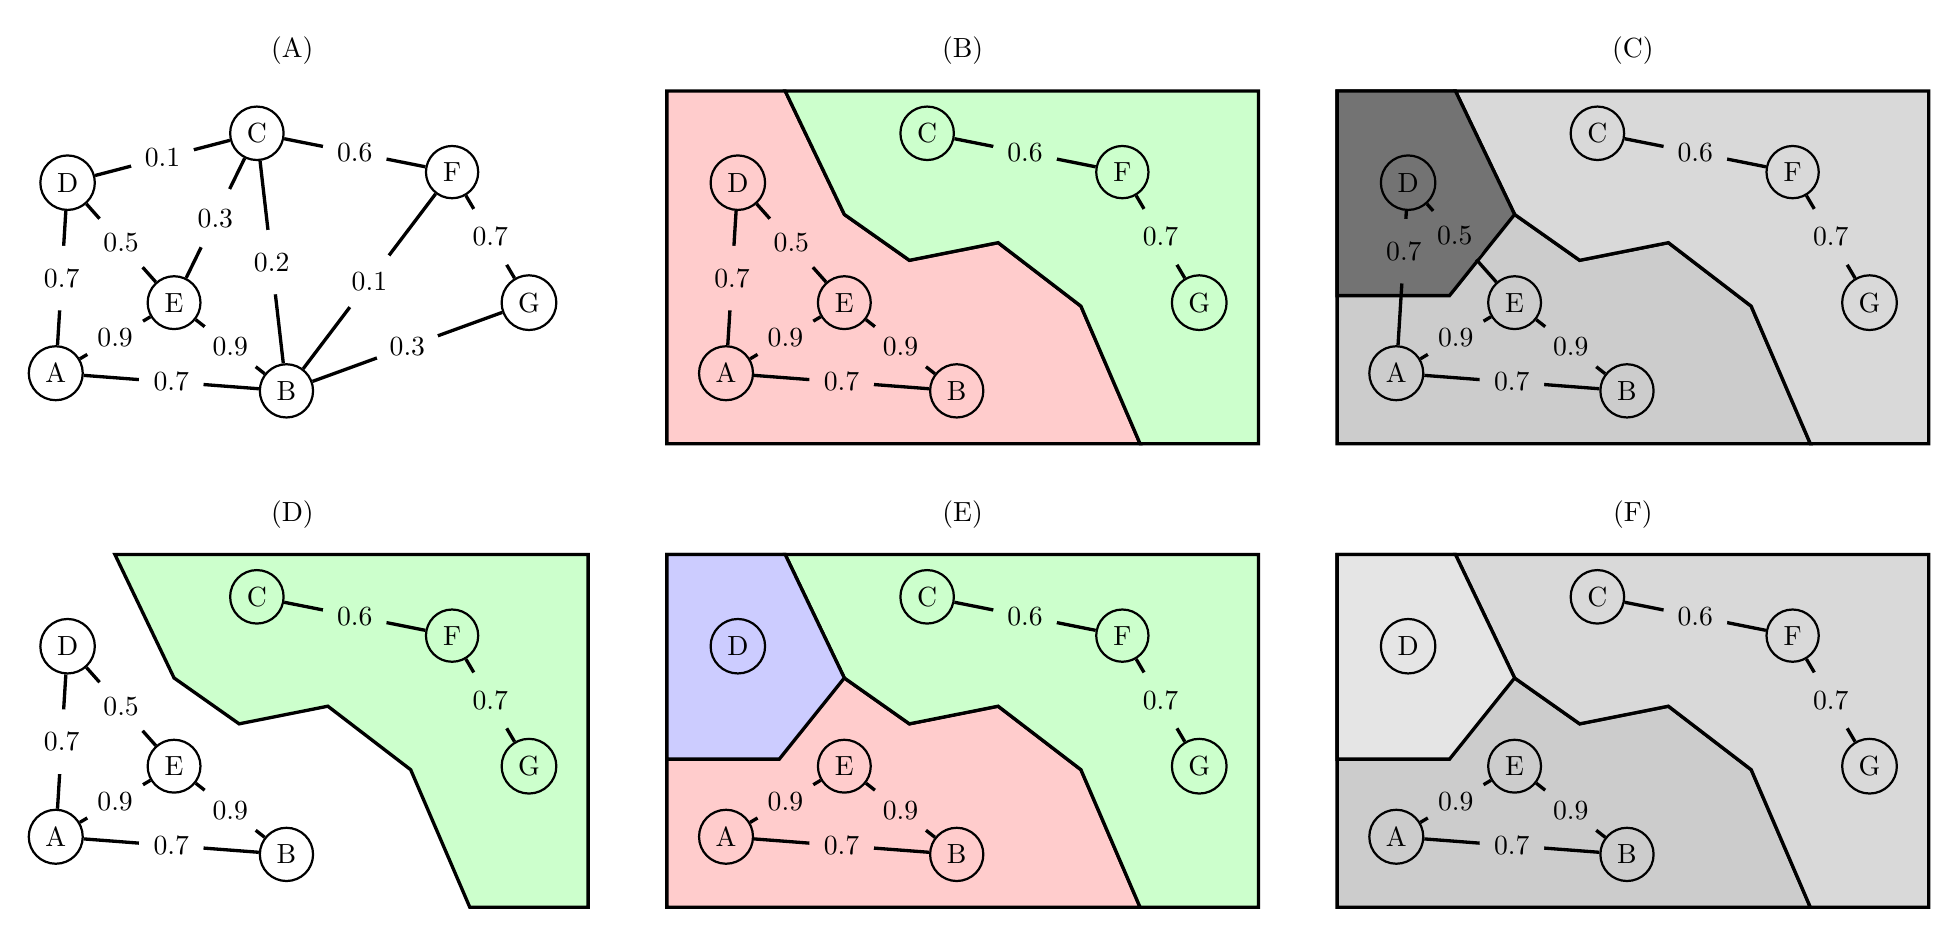
\begin{tikzpicture}
\begin{groupplot}[
	group style={
		group size=3 by 2,
		vertical sep=40pt
  	},
  	width=0.75\textwidth,
  	height=0.5\textwidth,
    no markers,
    axis lines*=left,
    every axis y label/.style={at=(current axis.above origin),anchor=south},
    every axis x label/.style={at=(current axis.right of origin),anchor=west},
    enlargelimits=false, clip=false, axis on top,
    hide axis, ytick=\empty, xtick=\empty,
    grid = major,
    xmin=0, xmax=10,
    ymin=0, ymax=10,
    auto title
	]

  %% ================================= 1:1 ==============================
\nextgroupplot[]
  \begin{scope}[every node/.style={circle,thick,draw}]
      \node (A) at (axis cs:1,2) {A};
      \node (B) at (axis cs:4.9,1.5) {B};
      \node (C) at (axis cs:4.4,8.8) {C};
      \node (D) at (axis cs:1.2,7.4) {D};
      \node (E) at (axis cs:3,4) {E};
      \node (F) at (axis cs:7.7,7.7) {F};
      \node (G) at (axis cs:9,4) {G};
  \end{scope}
  \begin{scope}[>={Stealth[black]},
                every node/.style={fill=white!20, circle},
                every edge/.style={draw=black, anchor=center, very thick}]
      \path [-] (A) edge node {$0.7$} (B);
      \path [-] (B) edge node {$0.2$} (C);
      \path [-] (C) edge node {$0.1$} (D);
      \path [-] (D) edge node {$0.7$} (A);
      \path [-] (A) edge node {$0.9$} (E);
      \path [-] (B) edge node {$0.9$} (E);
      \path [-] (C) edge node {$0.3$} (E);
      \path [-] (D) edge node {$0.5$} (E);
      \path [-] (B) edge node {$0.1$} (F); 
      \path [-] (C) edge node {$0.6$} (F); 
      \path [-] (B) edge node {$0.3$} (G); 
      \path [-] (F) edge node {$0.7$} (G); 
  \end{scope}

%% ================================= 1:2 ==============================
\nextgroupplot[]
      \coordinate (CDE) at (axis cs:3.0, 6.5) {};
      \coordinate (ADE) at (axis cs:1.9, 4.2) {};
      \coordinate (ABE) at (axis cs:2.6, 2.1) {};
      \coordinate (BCE) at (axis cs:4.1, 5.2) {};
      \coordinate (BCF) at (axis cs:5.6, 5.7) {};
      \coordinate (BFG) at (axis cs:7.0, 3.9) {};
      \coordinate (BG)  at (axis cs:8.0, 0.0) {};
      \coordinate (AD)  at (axis cs:0.0, 4.2) {};
      \coordinate (CD)  at (axis cs:2.0, 10.0) {};
      \coordinate (LL)  at (axis cs:0.0, 0.0) {};
      \coordinate (UL)  at (axis cs:10.0, 0.0) {};
      \coordinate (LU)  at (axis cs:0.0, 10.0) {};
      \coordinate (UU)  at (axis cs:10.0, 10.0) {};

      \draw[fill=red!20,very thick] (CD) -- (CDE) -- (BCE) -- (BCF) -- (BFG) -- (BG) -- (LL) -- (LU)-- cycle;
      \draw[fill=green!20,very thick] (CD) -- (CDE) -- (BCE) -- (BCF) -- (BFG) -- (BG) -- (UL) -- (UU)  -- cycle;

  \begin{scope}[every node/.style={circle,thick,draw}]
      \node (A) at (axis cs:1,2) {A};
      \node (B) at (axis cs:4.9,1.5) {B};
      \node (C) at (axis cs:4.4,8.8) {C};
      \node (D) at (axis cs:1.2,7.4) {D};
      \node (E) at (axis cs:3,4) {E};
      \node (F) at (axis cs:7.7,7.7) {F};
      \node (G) at (axis cs:9,4) {G};
  \end{scope}
  \begin{scope}[>={Stealth[black]},
                every node/.style={circle},
                every edge/.style={draw=black, very thick}]
      \path [-] (A) edge node [fill=red!20] {$0.7$} (B);
      \path [-] (D) edge node [fill=red!20] {$0.7$} (A);
      \path [-] (A) edge node [fill=red!20] {$0.9$} (E);
      \path [-] (B) edge node [fill=red!20] {$0.9$} (E);
      \path [-] (D) edge node [fill=red!20] {$0.5$} (E);

      \path [-] (C) edge node [fill=green!20] {$0.6$} (F); 
      \path [-] (F) edge node [fill=green!20] {$0.7$} (G); 
  \end{scope}

%% ================================= 1:3 ==============================
\nextgroupplot[]
      \coordinate (CDE) at (axis cs:3.0, 6.5) {};
      \coordinate (ADE) at (axis cs:1.9, 4.2) {};
      \coordinate (ABE) at (axis cs:2.6, 2.1) {};
      \coordinate (BCE) at (axis cs:4.1, 5.2) {};
      \coordinate (BCF) at (axis cs:5.6, 5.7) {};
      \coordinate (BFG) at (axis cs:7.0, 3.9) {};
      \coordinate (BG)  at (axis cs:8.0, 0.0) {};
      \coordinate (AD)  at (axis cs:0.0, 4.2) {};
      \coordinate (CD)  at (axis cs:2.0, 10.0) {};
      \coordinate (LL)  at (axis cs:0.0, 0.0) {};
      \coordinate (UL)  at (axis cs:10.0, 0.0) {};
      \coordinate (LU)  at (axis cs:0.0, 10.0) {};
      \coordinate (UU)  at (axis cs:10.0, 10.0) {};

      \draw[fill=black!20,very thick] (CD) -- (CDE) -- (BCE) -- (BCF) -- (BFG) -- (BG) -- (LL) -- (LU)-- cycle;
      \draw[fill=black!15,very thick] (CD) -- (CDE) -- (BCE) -- (BCF) -- (BFG) -- (BG) -- (UL) -- (UU)  -- cycle;
      \draw[fill=black!55,very thick] (CD) -- (CDE) -- (ADE) -- (AD) -- (LU)-- cycle;

  \begin{scope}[every node/.style={circle,thick,draw}]
      \node (A) at (axis cs:1,2) {A};
      \node (B) at (axis cs:4.9,1.5) {B};
      \node (C) at (axis cs:4.4,8.8) {C};
      \node (D) at (axis cs:1.2,7.4) {D};
      \node (E) at (axis cs:3,4) {E};
      \node (F) at (axis cs:7.7,7.7) {F};
      \node (G) at (axis cs:9,4) {G};
  \end{scope}
  \begin{scope}[>={Stealth[black]},
                every node/.style={circle},
                every edge/.style={draw=black, very thick}]
      \path [-] (A) edge node [fill=black!20] {$0.7$} (B);
      \path [-] (A) edge node [fill=black!20] {$0.9$} (E);
      \path [-] (B) edge node [fill=black!20] {$0.9$} (E);
      
      \path [-] (D) edge node [fill=black!55, pos=0.3] {$0.7$} (A);
      \path [-] (D) edge node [fill=black!55, pos=0.4] {$0.5$} (E);

      \path [-] (C) edge node [fill=black!15] {$0.6$} (F); 
      \path [-] (F) edge node [fill=black!15] {$0.7$} (G); 
  \end{scope}

%% ================================= 2:1 ==============================
\nextgroupplot[]
      \coordinate (CDE) at (axis cs:3.0, 6.5) {};
      \coordinate (ADE) at (axis cs:1.9, 4.2) {};
      \coordinate (ABE) at (axis cs:2.6, 2.1) {};
      \coordinate (BCE) at (axis cs:4.1, 5.2) {};
      \coordinate (BCF) at (axis cs:5.6, 5.7) {};
      \coordinate (BFG) at (axis cs:7.0, 3.9) {};
      \coordinate (BG)  at (axis cs:8.0, 0.0) {};
      \coordinate (AD)  at (axis cs:0.0, 4.2) {};
      \coordinate (CD)  at (axis cs:2.0, 10.0) {};
      \coordinate (LL)  at (axis cs:0.0, 0.0) {};
      \coordinate (UL)  at (axis cs:10.0, 0.0) {};
      \coordinate (LU)  at (axis cs:0.0, 10.0) {};
      \coordinate (UU)  at (axis cs:10.0, 10.0) {};

      \draw[fill=green!20,very thick] (CD) -- (CDE) -- (BCE) -- (BCF) -- (BFG) -- (BG) -- (UL) -- (UU)  -- cycle;

  \begin{scope}[every node/.style={circle,thick,draw}]
      \node (A) at (axis cs:1,2) {A};
      \node (B) at (axis cs:4.9,1.5) {B};
      \node (C) at (axis cs:4.4,8.8) {C};
      \node (D) at (axis cs:1.2,7.4) {D};
      \node (E) at (axis cs:3,4) {E};
      \node (F) at (axis cs:7.7,7.7) {F};
      \node (G) at (axis cs:9,4) {G};
  \end{scope}
  \begin{scope}[>={Stealth[black]},
                every node/.style={circle, fill=white},
                every edge/.style={draw=black, very thick}]
      \path [-] (A) edge node {$0.7$} (B);
      \path [-] (D) edge node {$0.7$} (A);
      \path [-] (A) edge node {$0.9$} (E);
      \path [-] (B) edge node {$0.9$} (E);
      \path [-] (D) edge node {$0.5$} (E);

      \path [-] (C) edge node [fill=green!20] {$0.6$} (F); 
      \path [-] (F) edge node [fill=green!20] {$0.7$} (G); 
  \end{scope}
  
%% ================================= 2:2 ==============================
\nextgroupplot[]
      \coordinate (CDE) at (axis cs:3.0, 6.5) {};
      \coordinate (ADE) at (axis cs:1.9, 4.2) {};
      \coordinate (ABE) at (axis cs:2.6, 2.1) {};
      \coordinate (BCE) at (axis cs:4.1, 5.2) {};
      \coordinate (BCF) at (axis cs:5.6, 5.7) {};
      \coordinate (BFG) at (axis cs:7.0, 3.9) {};
      \coordinate (BG)  at (axis cs:8.0, 0.0) {};
      \coordinate (AD)  at (axis cs:0.0, 4.2) {};
      \coordinate (CD)  at (axis cs:2.0, 10.0) {};
      \coordinate (LL)  at (axis cs:0.0, 0.0) {};
      \coordinate (UL)  at (axis cs:10.0, 0.0) {};
      \coordinate (LU)  at (axis cs:0.0, 10.0) {};
      \coordinate (UU)  at (axis cs:10.0, 10.0) {};

      \draw[fill=red!20,very thick] (CD) -- (CDE) -- (BCE) -- (BCF) -- (BFG) -- (BG) -- (LL) -- (LU)-- cycle;
      \draw[fill=green!20,very thick] (CD) -- (CDE) -- (BCE) -- (BCF) -- (BFG) -- (BG) -- (UL) -- (UU)  -- cycle;
      \draw[fill=blue!20,very thick] (CD) -- (CDE) -- (ADE) -- (AD) -- (LU)-- cycle;

  \begin{scope}[every node/.style={circle,thick,draw}]
      \node (A) at (axis cs:1,2) {A};
      \node (B) at (axis cs:4.9,1.5) {B};
      \node (C) at (axis cs:4.4,8.8) {C};
      \node (D) at (axis cs:1.2,7.4) {D};
      \node (E) at (axis cs:3,4) {E};
      \node (F) at (axis cs:7.7,7.7) {F};
      \node (G) at (axis cs:9,4) {G};
  \end{scope}
  \begin{scope}[>={Stealth[black]},
                every node/.style={circle},
                every edge/.style={draw=black, very thick}]
      \path [-] (A) edge node [fill=red!20] {$0.7$} (B);
      \path [-] (A) edge node [fill=red!20] {$0.9$} (E);
      \path [-] (B) edge node [fill=red!20] {$0.9$} (E);

      \path [-] (C) edge node [fill=green!20] {$0.6$} (F); 
      \path [-] (F) edge node [fill=green!20] {$0.7$} (G); 
  \end{scope}
  
%% ================================= 2:3 ==============================
\nextgroupplot[]
      \coordinate (CDE) at (axis cs:3.0, 6.5) {};
      \coordinate (ADE) at (axis cs:1.9, 4.2) {};
      \coordinate (ABE) at (axis cs:2.6, 2.1) {};
      \coordinate (BCE) at (axis cs:4.1, 5.2) {};
      \coordinate (BCF) at (axis cs:5.6, 5.7) {};
      \coordinate (BFG) at (axis cs:7.0, 3.9) {};
      \coordinate (BG)  at (axis cs:8.0, 0.0) {};
      \coordinate (AD)  at (axis cs:0.0, 4.2) {};
      \coordinate (CD)  at (axis cs:2.0, 10.0) {};
      \coordinate (LL)  at (axis cs:0.0, 0.0) {};
      \coordinate (UL)  at (axis cs:10.0, 0.0) {};
      \coordinate (LU)  at (axis cs:0.0, 10.0) {};
      \coordinate (UU)  at (axis cs:10.0, 10.0) {};

      \draw[fill=black!20,very thick] (CD) -- (CDE) -- (BCE) -- (BCF) -- (BFG) -- (BG) -- (LL) -- (LU)-- cycle;
      \draw[fill=black!15,very thick] (CD) -- (CDE) -- (BCE) -- (BCF) -- (BFG) -- (BG) -- (UL) -- (UU)  -- cycle;
      \draw[fill=black!10,very thick] (CD) -- (CDE) -- (ADE) -- (AD) -- (LU)-- cycle;

  \begin{scope}[every node/.style={circle,thick,draw}]
      \node (A) at (axis cs:1,2) {A};
      \node (B) at (axis cs:4.9,1.5) {B};
      \node (C) at (axis cs:4.4,8.8) {C};
      \node (D) at (axis cs:1.2,7.4) {D};
      \node (E) at (axis cs:3,4) {E};
      \node (F) at (axis cs:7.7,7.7) {F};
      \node (G) at (axis cs:9,4) {G};
  \end{scope}
  \begin{scope}[>={Stealth[black]},
                every node/.style={circle},
                every edge/.style={draw=black, very thick}]
      \path [-] (A) edge node [fill=black!20] {$0.7$} (B);
      \path [-] (A) edge node [fill=black!20] {$0.9$} (E);
      \path [-] (B) edge node [fill=black!20] {$0.9$} (E);

      \path [-] (C) edge node [fill=black!15] {$0.6$} (F); 
      \path [-] (F) edge node [fill=black!15] {$0.7$} (G); 
  \end{scope}

\end{groupplot} 
\end{tikzpicture}
\end{document}